\chapter{Manual del desarrollador}

\section{Mecanismo de adición de vistas}

La aplicación ha sido diseñada para permitir añadir nuevas vistas para propiedades y dispositivos sin la necesidad de conocer el código de la aplicación. Cualquier clase que se añada debe ir dentro del paquete principal con el resto de clases. Igualmente, todos los layaout de android (vistas) deben ir en la carpeta de \texttt{resources} y dentro de esta en \texttt{layouts}.

\bigskip
\subsection{Propiedades}
Para poder añadir una nueva vista debemos seguir tres pasos:

\begin{itemize}
  \item Crear una clase que implemente la interfaz \textbf{UIPropertyManager}.
  \item Crear una interfaz de usuario para android en XML tanto para la vista de elemento de lista como para la vista para editar una propiedad.
  \item Declarar un objeto de la clase creada y añadirlo al vector de manejadores.
\end{itemize}


\subsubsection{Interfaz UIPropertyManager}

A continuación se muestra la interfaz de Java que debemos implementar en la nueva clase manejadora que deseamos crear.

\begin{lstlisting}[language=Java,caption={Interfaz UIPropertyManager},label={lst:ui_prop_manager}]

/**
 *  Interface to handle views and indi propertys
 */
public interface UIPropertyManager {
    /**
     *  Check if this class can represent p
     *
     * @param p Indi property
     * @return True/false if class can represent p
     */
    boolean handlesProperty (INDIProperty p);

    /**
     *  Create and return a view sets with p elements
     *
     * @param p Indi property
     * @param inflater Layout inflater to inflate view
     * @param parent ViewGroup to inflate view
     * @param context Context to allow use Activity methods
     * @return View
     */
    View getPropertyView (INDIProperty p, LayoutInflater inflater, ViewGroup parent, Context context);

    /**
     *  update view v with Indi property p elements
     *
     * @param p Indi property
     * @param v View
     */
    void updateView (INDIProperty p, View v);

    /**
     *  Create a new view dialog to allow set Indi property p elements
     *
     * @param p Indi property
     * @param inflater Layout inflater to inflate view
     * @return View
     */
    View getUpdateView(INDIProperty p, LayoutInflater inflater, DialogFragment fragment);

    /**
     *  Update property with change saved at view v
     *
     * @param p Indi property
     * @param v View
     */
    void updateProperty(INDIProperty p, View v);

    /**
     *  Get priority
     *
     * @return priority
     */
    int getPriority();

    /**
     *  Get update button reference
     *
     *  @return update button
     */

    Button getUpdateButton();
}

\end{lstlisting}

\bigskip
Como podemos ver en el fragmento de código \ref{lst:ui_prop_manager}, las funciones que debemos implementar son:

\begin{itemize}
  \item \texttt{handlesProperty}:
  Esta función recibe una propiedad y debe comprobar si puede manejarla o no devolviendo un valor booleano.

  \item \texttt{getPropertyView}:
  Una vez que comprobamos que podemos manejar la propiedad, esta función debe devolvernos la vista ``inflada'' que se mostrará en la lista de propiedades. Los parámetros \tetxit{inflater, parent y context} son necesarios para poder inflar la vista.

  \item \texttt{updateView}:
  Esta función es la que debe coger la vista anteriormente creada, y debe rellenarla a partir de la propiedad p.

  \item \texttt{getUpdateView}:
  Esta función debe crear la vista para el modo de edición de la propiedad. Esta vista se pintará en un diálogo de tipo \texttt{Fragment}. Al igual que antes, necesitamos las variables \tetxit{inflater y fragment} para ``inflar'' la vista.

  \item \texttt{updateProperty}:
  La vista para editar propiedades permite al usuario editar una propiedad. Una vez que el usuario ha terminado la edición, debemos actualizar la propiedad con los valores de la vista y enviar la información al servidor usando la función de la propiedad de \textbf{INDI}, \texttt{sendChangesToDriver}. 

  \item \texttt{getPriority}:
  Esta función debe devolver una valor numérico para establecer la prioridad que tendrá la vista respecto a otras vistas o a la vista por defecto de la propiedad. Cuanto mayor sea el valor, más prioridad tendrá

  \item \texttt{getUpdateButton}:
  Esta función debe devolver un objeto ``Button'' si la vista tendrá el botón para actualizar, o \textit{null} en caso de que no haya botón.
\end{itemize}

Para ilustrar la creación de la clase y la implementaicón de la interfaz, en el segmento de código \ref{lst:connect_class} podemos ver la implementación de la clase \texttt{UIConnecPropertyManager}. Este tipo de propiedad es una \textit{Switch} al que se va a cambiar la vista por defecto. Vemos que es muy importante implementar la función \texttt{handlesProperty} ya que en ella debemos comprobar si la propiedad que nos mandan es la que podemos manejar. 

\bigskip
Otro ejemplo de clase manejadora es la del segmento de código \ref{lst:abort_class}. En este caso buscamos cualquier propiedad de tipo \textit{switch} que tenga un solo elemento y que su nombre sea ``Abort''.

\begin{lstlisting}[language=Java,caption={Clase manejadora de la propiedad connection},label={lst:connect_class}]
public class UIConnecPropertyManager implements UIPropertyManager,View.OnClickListener {
    //Atributes
    int layout;
    int layout_dialog;
    Button button;

    public UIConnecPropertyManager(){
        layout=R.layout.connec_property_view_list_item;
        layout_dialog=R.layout.connec_property_edit_view;
    }

    @Override
    public boolean handlesProperty(INDIProperty p) {

        if(p.getName().equals("CONNECTION"))
            return true;
        else
            return false;
    }

    @Override
    public View getPropertyView(INDIProperty p, LayoutInflater inflater, ViewGroup parent, Context context) {
        View v=inflater.inflate(layout, parent, false);
        return v;
    }


    @Override
    public void updateView(INDIProperty p, View v) {
        setView(v, p);
    }

    @Override
    public View getUpdateView(INDIProperty p, LayoutInflater inflater, DialogFragment fragment) {
        View v = inflater.inflate(layout_dialog,null);
        TextView name=(TextView)v.findViewById(R.id.property_name);
        Switch s=(Switch)v.findViewById(R.id.conn_switch);
        button=(Button)v.findViewById(R.id.update_button);

        ArrayList<INDIElement> list =(ArrayList) p.getElementsAsList();
        INDISwitchElement elem=(INDISwitchElement)list.get(0);

        if (elem.getValue().equals(Constants.SwitchStatus.ON))
            s.setChecked(true);
        else
            s.setChecked(false);

        name.setText(p.getLabel());
        return v;
    }


    @Override
    public void updateProperty(INDIProperty p, View v) {
        Switch s=(Switch)v.findViewById(R.id.conn_switch);

        ArrayList<INDIElement> list =(ArrayList) p.getElementsAsList();
        INDISwitchElement conect=(INDISwitchElement)list.get(0);
        INDISwitchElement disconect=(INDISwitchElement)list.get(1);

        try {
            if(s.isChecked()){
                disconect.setDesiredValue(Constants.SwitchStatus.OFF);
                conect.setDesiredValue(Constants.SwitchStatus.ON);
            }else{
                disconect.setDesiredValue(Constants.SwitchStatus.ON);
                conect.setDesiredValue(Constants.SwitchStatus.OFF);
            }

        p.sendChangesToDriver();

        } catch (INDIValueException e) {
            e.printStackTrace();
        } catch (IOException e) {
            e.printStackTrace();
        }
    }

    @Override
    public int getPriority() {
        return 5;
    }

    @Override
    public Button getUpdateButton() {
        return button;
    }

    void setView(View v, INDIProperty p){
        //Views
        TextView name = (TextView)v.findViewById(R.id.name);
        ImageView idle = (ImageView)v.findViewById(R.id.idle);
        TextView perm = (TextView)v.findViewById(R.id.perm);
        ImageView visibility = (ImageView)v.findViewById(R.id.visibility);
        TextView element = (TextView)v.findViewById(R.id.element);

        visibility.setTag(p);
        visibility.setFocusable(false);
        visibility.setOnClickListener(this);

        //others
        int light_res=0;
        String perm_res="";
        int visibility_res=0;

        ArrayList<INDIElement> list =(ArrayList) p.getElementsAsList();

        String text="";

        INDISwitchElement elem=(INDISwitchElement)list.get(0);

        if (elem.getValue().equals(Constants.SwitchStatus.ON))
            text="Connected";
        else
            text="Disconnected";

        element.setText(text);


        //State
        if(p.getState().name().equals("IDLE")){
            light_res=R.drawable.grey_light_48;
        }else if(p.getState().name().equals("OK")){
            light_res=R.drawable.green_light_48;
        }else if(p.getState().name().equals("BUSY")){
            light_res=R.drawable.yellow_light_48;
        }else{
            light_res=R.drawable.red_light_48;
        }

        //Permission
        if(p.getPermission().equals(Constants.PropertyPermissions.RO)){
            perm_res="RO";
        }else if(p.getPermission().equals(Constants.PropertyPermissions.WO)){
            perm_res="WO";
        }else{
            perm_res="RW";
        }

        if(DefaultDeviceView.conn.isPropertyHide(p))
            visibility_res=R.drawable.ic_visibility_off_black_24dp;
        else
            visibility_res=R.drawable.ic_visibility_black_24dp;


        name.setText(p.getLabel());
        idle.setImageResource(light_res);
        perm.setText(perm_res);
        visibility.setImageResource(visibility_res);
    }

    @Override
    public void onClick(View v) {
        INDIProperty p=(INDIProperty)v.getTag();
        Connection conn=DefaultDeviceView.conn;
        if(conn.isPropertyHide(p)){
            conn.showProperty(p);
        }else{
            conn.hideProperty(p);
        }
    }
}

\end{lstlisting}

\begin{lstlisting}[language=Java,caption={Clase manejadora de propiedades Abort},label={lst:abort_class}]
public abstract class DeviceView extends Fragment {

public class UIAbortPropertyManager implements UIPropertyManager,View.OnClickListener {

    //Atributes
    int layout;
    int layout_dialog;
    Button button;
    Context context;

    public UIAbortPropertyManager(){
        layout=R.layout.abort_property_view_list_item;
        layout_dialog=R.layout.abort_property_edit_view;
    }

    @Override
    public boolean handlesProperty(INDIProperty p) {
        if(p instanceof INDISwitchProperty){
            ArrayList<INDIElement> list =(ArrayList) p.getElementsAsList();
            if(list.size()==1) {
                INDISwitchElement elem = (INDISwitchElement) list.get(0);
                if(elem.getLabel().equals("Abort")){
                    return true;
                }
                else{
                    return false;
                }
            }else{
                return false;
            }
        }else{
            return false;
        }
    }

    @Override
    public View getPropertyView(INDIProperty p, LayoutInflater inflater, ViewGroup parent, Context context) {
        this.context=context;
        View v=inflater.inflate(layout, parent, false);
        return v;
    }

    @Override
    public void updateView(INDIProperty p, View v) {
        setView(v, p);
    }

    @Override
    public View getUpdateView(INDIProperty p, LayoutInflater inflater, DialogFragment fragment) {
        View v = inflater.inflate(layout_dialog,null);
        TextView name=(TextView)v.findViewById(R.id.property_name);
        button=(Button)v.findViewById(R.id.abort_button);
        name.setText(p.getLabel());
        return v;
    }

    @Override
    public void updateProperty(INDIProperty p, View v) {
        ArrayList<INDIElement> list =(ArrayList) p.getElementsAsList();
        INDISwitchElement abort=(INDISwitchElement)list.get(0);

        try {
            abort.setDesiredValue(Constants.SwitchStatus.ON);
            p.sendChangesToDriver();
        } catch (INDIValueException e) {
            e.printStackTrace();
        } catch (IOException e) {
            e.printStackTrace();
        }
    }

    @Override
    public int getPriority() {
        return 9;
    }

    @Override
    public Button getUpdateButton() {
        return button;
    }

    void setView(View v, INDIProperty p){
        //Views
        TextView name = (TextView)v.findViewById(R.id.name);
        ImageView idle = (ImageView)v.findViewById(R.id.idle);
        TextView perm = (TextView)v.findViewById(R.id.perm);
        ImageView visibility = (ImageView)v.findViewById(R.id.visibility);
        TextView element = (TextView)v.findViewById(R.id.element);

        visibility.setTag(p);
        visibility.setFocusable(false);
        visibility.setOnClickListener(this);

        //others
        int light_res=0;
        String perm_res="";
        int visibility_res=0;

        String text=context.getResources().getString(R.string.abort_text);

        element.setText(Html.fromHtml("<strong><font color=\"red\"><u>"+text+"</u></font></strong>"));


        //State
        if(p.getState().name().equals("IDLE")){
            light_res=R.drawable.grey_light_48;
        }else if(p.getState().name().equals("OK")){
            light_res=R.drawable.green_light_48;
        }else if(p.getState().name().equals("BUSY")){
            light_res=R.drawable.yellow_light_48;
        }else{
            light_res=R.drawable.red_light_48;
        }

        //Permission
        if(p.getPermission().equals(Constants.PropertyPermissions.RO)){
            perm_res="RO";
        }else if(p.getPermission().equals(Constants.PropertyPermissions.WO)){
            perm_res="WO";
        }else{
            perm_res="RW";
        }

        if(DefaultDeviceView.conn.isPropertyHide(p))
            visibility_res=R.drawable.ic_visibility_off_black_24dp;
        else
            visibility_res=R.drawable.ic_visibility_black_24dp;


        name.setText(p.getLabel());
        idle.setImageResource(light_res);
        perm.setText(perm_res);
        visibility.setImageResource(visibility_res);
    }

    @Override
    public void onClick(View v) {
        INDIProperty p=(INDIProperty)v.getTag();
        Connection conn=DefaultDeviceView.conn;
        if(conn.isPropertyHide(p)){
            conn.showProperty(p);
        }else{
            conn.hideProperty(p);
        }
    }
}

\end{lstlisting}

\bigskip
Una vez que tenemos la clase creada debemos diseñar la interfaz de usuario en un archivo \textit{XML} como el del archivo del fragmento de código \ref{lst:xml_item_view} que representa la vista de elemento de lista de la propiedad \textit{Connection}. Además de este, debemos crear otra vista para mostrar en el diálogo de edición de propiedades (fragmento de código \ref{}). No hay ningún tipo de restricción para estas vistas. El desarrollador es libre de poner lo que necesite en ambas interfaces de usuario.

\begin{lstlisting}[language=XML,caption={Vista item XML de una propiedad},label={lst:xml_item_view}]
<?xml version="1.0" encoding="utf-8"?>

<RelativeLayout xmlns:android="http://schemas.android.com/apk/res/android"
    android:layout_width="match_parent" android:layout_height="wrap_content"
    android:padding="5dp">

    <ImageView
        android:layout_width="wrap_content"
        android:layout_height="wrap_content"
        android:id="@+id/idle"
        android:layout_marginRight="10dp"
        android:layout_alignParentLeft="true" />

    <TextView
        android:layout_width="wrap_content"
        android:layout_height="wrap_content"
        android:text="New Text"
        android:id="@+id/name"
        android:layout_alignParentTop="true"
        android:layout_toRightOf="@+id/idle"
        android:layout_marginLeft="10dp"
        android:textAppearance="@android:style/TextAppearance.Holo.Large"
        android:textStyle="bold" />
    <TextView
        android:layout_width="wrap_content"
        android:layout_height="wrap_content"
        android:text=""
        android:id="@+id/label"
        android:layout_below="@+id/name"
        android:layout_toRightOf="@+id/idle"
        android:layout_marginTop="10dp"
        android:layout_marginLeft="10dp"
        android:textAppearance="@android:style/TextAppearance.Holo.Medium" />

    <TextView
        android:layout_width="wrap_content"
        android:layout_height="wrap_content"
        android:text=""
        android:id="@+id/type"
        android:layout_below="@+id/label"
        android:layout_toRightOf="@+id/idle"
        android:layout_marginTop="10dp"
        android:layout_marginLeft="10dp"
        android:textAppearance="@android:style/TextAppearance.Holo.Medium" />

    <ImageButton
        android:layout_width="wrap_content"
        android:layout_height="wrap_content"
        android:layout_margin="30dp"
        android:src="@drawable/ic_save_black_24dp"
        android:id="@+id/save_button"
        android:layout_below="@+id/type"
        android:layout_toRightOf="@+id/idle"/>

    <ImageButton
        android:layout_width="wrap_content"
        android:layout_height="wrap_content"
        android:src="@drawable/ic_pageview_black_24dp"
        android:id="@+id/view_button"
        android:layout_alignTop="@+id/save_button"
        android:layout_toRightOf="@+id/save_button"
        android:layout_toEndOf="@+id/save_button" />

    <TextView
        android:layout_width="wrap_content"
        android:layout_height="wrap_content"
        android:id="@+id/perm"
        android:textStyle="bold"
        android:text=""
        android:layout_margin="8dp"
        android:paddingTop="10dp"
        android:paddingLeft="4dp"
        android:layout_alignParentLeft="true"
        android:layout_below="@+id/idle"
        android:textColor="#ff000000" />

    <ImageView
        android:layout_width="wrap_content"
        android:layout_height="wrap_content"
        android:id="@+id/visibility"
        android:layout_margin="10dp"
        android:layout_alignParentLeft="true"
        android:layout_below="@+id/perm"/>

</RelativeLayout>


\end{lstlisting}

\begin{lstlisting}[language=XML,caption={Vista de edición  XML de una propiedad},label={lst:lst:xml_edit_view}]

<?xml version="1.0" encoding="utf-8"?>
<ScrollView xmlns:android="http://schemas.android.com/apk/res/android"
    android:id="@+id/ScrollView01"
    android:layout_width="fill_parent"
    android:layout_height="fill_parent">
<RelativeLayout xmlns:android="http://schemas.android.com/apk/res/android"
    android:layout_width="match_parent"
    android:layout_height="match_parent"
    android:background="@android:color/white"
    android:padding="24dp">


    <TextView
        android:id="@+id/info_text"
        android:layout_width="wrap_content"
        android:layout_height="wrap_content"
        android:layout_alignParentTop="true"
        android:layout_centerHorizontal="true"
        android:gravity="center"
        android:text="@string/action_edit"
        android:textSize="20dp" />


    <View
        android:id="@+id/divider"
        android:layout_width="match_parent"
        android:layout_height="1dp"
        android:layout_below="@+id/info_text"
        android:layout_marginBottom="20dp"
        android:layout_marginTop="10dp"
        android:background="#C8C9CB" />

    <EditText
        android:id="@+id/name"
        android:layout_width="match_parent"
        android:layout_height="wrap_content"
        android:layout_below="@+id/divider"
        android:layout_centerHorizontal="true"
        android:layout_marginTop="20dp"
        android:background="@drawable/text_border"
        android:ems="10"
        android:hint="@string/hint_name"
        android:inputType="textUri"
        android:padding="12dp"
        android:textAppearance="?android:attr/textAppearanceSmall"
        android:textSize="18dp"
        android:textColor="#346D7D"
        android:text="indiserver" />

    <EditText
        android:id="@+id/host"
        android:layout_width="match_parent"
        android:layout_height="wrap_content"
        android:layout_below="@+id/name"
        android:layout_centerHorizontal="true"
        android:layout_marginTop="20dp"
        android:background="@drawable/text_border"
        android:ems="10"
        android:hint="@string/hint_host"
        android:inputType="textUri"
        android:padding="12dp"
        android:textAppearance="?android:attr/textAppearanceSmall"
        android:textSize="18dp"
        android:textColor="#346D7D"
        android:text="indiserver.no-ip.org" />

    <EditText
        android:id="@+id/port"
        android:layout_width="match_parent"
        android:layout_height="wrap_content"
        android:layout_below="@+id/host"
        android:layout_centerHorizontal="true"
        android:layout_marginBottom="20dp"
        android:layout_marginTop="20dp"
        android:background="@drawable/text_border"
        android:ems="10"
        android:hint="@string/hint_port"
        android:inputType="number"
        android:padding="12dp"
        android:textAppearance="?android:attr/textAppearanceSmall"
        android:textSize="18dp"
        android:textColor="#346D7D"
        android:text="7624" />

    <Switch
        android:layout_width="match_parent"
        android:layout_height="wrap_content"
        android:layout_centerHorizontal="true"
        android:text="@string/autoconnect"
        android:layout_marginRight="20dp"
        android:layout_marginLeft="20dp"
        android:layout_marginBottom="20dp"
        android:layout_below="@+id/port"
        android:id="@+id/autconnect" />

    <Switch
        android:layout_width="match_parent"
        android:layout_height="wrap_content"
        android:layout_centerHorizontal="true"
        android:text="@string/blob_enable"
        android:layout_marginRight="20dp"
        android:layout_marginLeft="20dp"
        android:layout_marginBottom="20dp"
        android:layout_below="@+id/autconnect"
        android:id="@+id/blob_recive" />


    <Button
        android:id="@+id/remove_log_button"
        android:layout_width="wrap_content"
        android:layout_height="wrap_content"
        android:padding="10dp"
        android:layout_marginBottom="30dp"
        android:layout_marginTop="15dp"
        android:text="@string/remove_log"
        android:textSize="14dp"
        android:layout_below="@+id/blob_recive"
        android:layout_centerHorizontal="true"
        android:enabled="false" />


    <Button
        android:id="@+id/edit_button"
        android:layout_width="match_parent"
        android:layout_height="wrap_content"
        android:paddingBottom="20dp"
        android:paddingTop="20dp"
        android:layout_marginBottom="20dp"
        android:text="@string/edit_connect"
        android:textColor="@android:color/white"
        android:background="#346D7D"
        android:layout_alignParentLeft="true"
        android:layout_alignParentStart="true"
        android:textSize="18dp"
        android:layout_below="@+id/remove_log_button" />


</RelativeLayout>
    </ScrollView>

\end{lstlisting}


\bigskip
Una vez creada la clase y las dos vistas en archivos XML, debemos añadir un objeto de la nueva clase manejadora, a la lista con el resto de objetos para manejar propiedades. Según la prioridad establecida, el nuevo manejador de propiedades se colocarán en una posición concreta. En el segmento de código \ref{lst:property_uis} podemos ver esta lista. La función que se observa es llamada al inicio del programa para establecer todas las clases que pueden manejar propiedades. Para cada objeto, llamamos al método de la clase \texttt{Config} \texttt{addUiPropertyManager(nuevo manejador)}

\begin{lstlisting}[language=Java,caption={Lista de objetos manejadores de propiedades},label={lst:property_uis}]

private void setUiProperties() {
        //add UI object
        Config.init();
        Config.addUiPropertyManager(new UIBlobPropertyManager());
        Config.addUiPropertyManager(new UITextPropertyManager());
        Config.addUiPropertyManager(new UISwitchPropertyManager());
        Config.addUiPropertyManager(new UINumberPropertyManager());
        Config.addUiPropertyManager(new UILightPropertyManager());
        Config.addUiPropertyManager(new UIConnecPropertyManager());
        Config.addUiPropertyManager(new UIAbortPropertyManager());

    }

\end{lstlisting}

Este método se encuentra definido en la actividad principal que se encuentra en el archivo ``MainActivity.java''. Debemos buscarla y añadir ahí el objeto de nuestra clase.

\bigskip
En la figura \ref{fig:connect_abort} podemos ver la vista de las propiedades \texttt{Connection} y \texttt{Abort} en la lista, y en las figuras \ref{fig:connect_edit_view} y \ref{fig:abort_edit_view}, sus vistas de edición

\begin{figure}[!ht]
  \begin{center}
  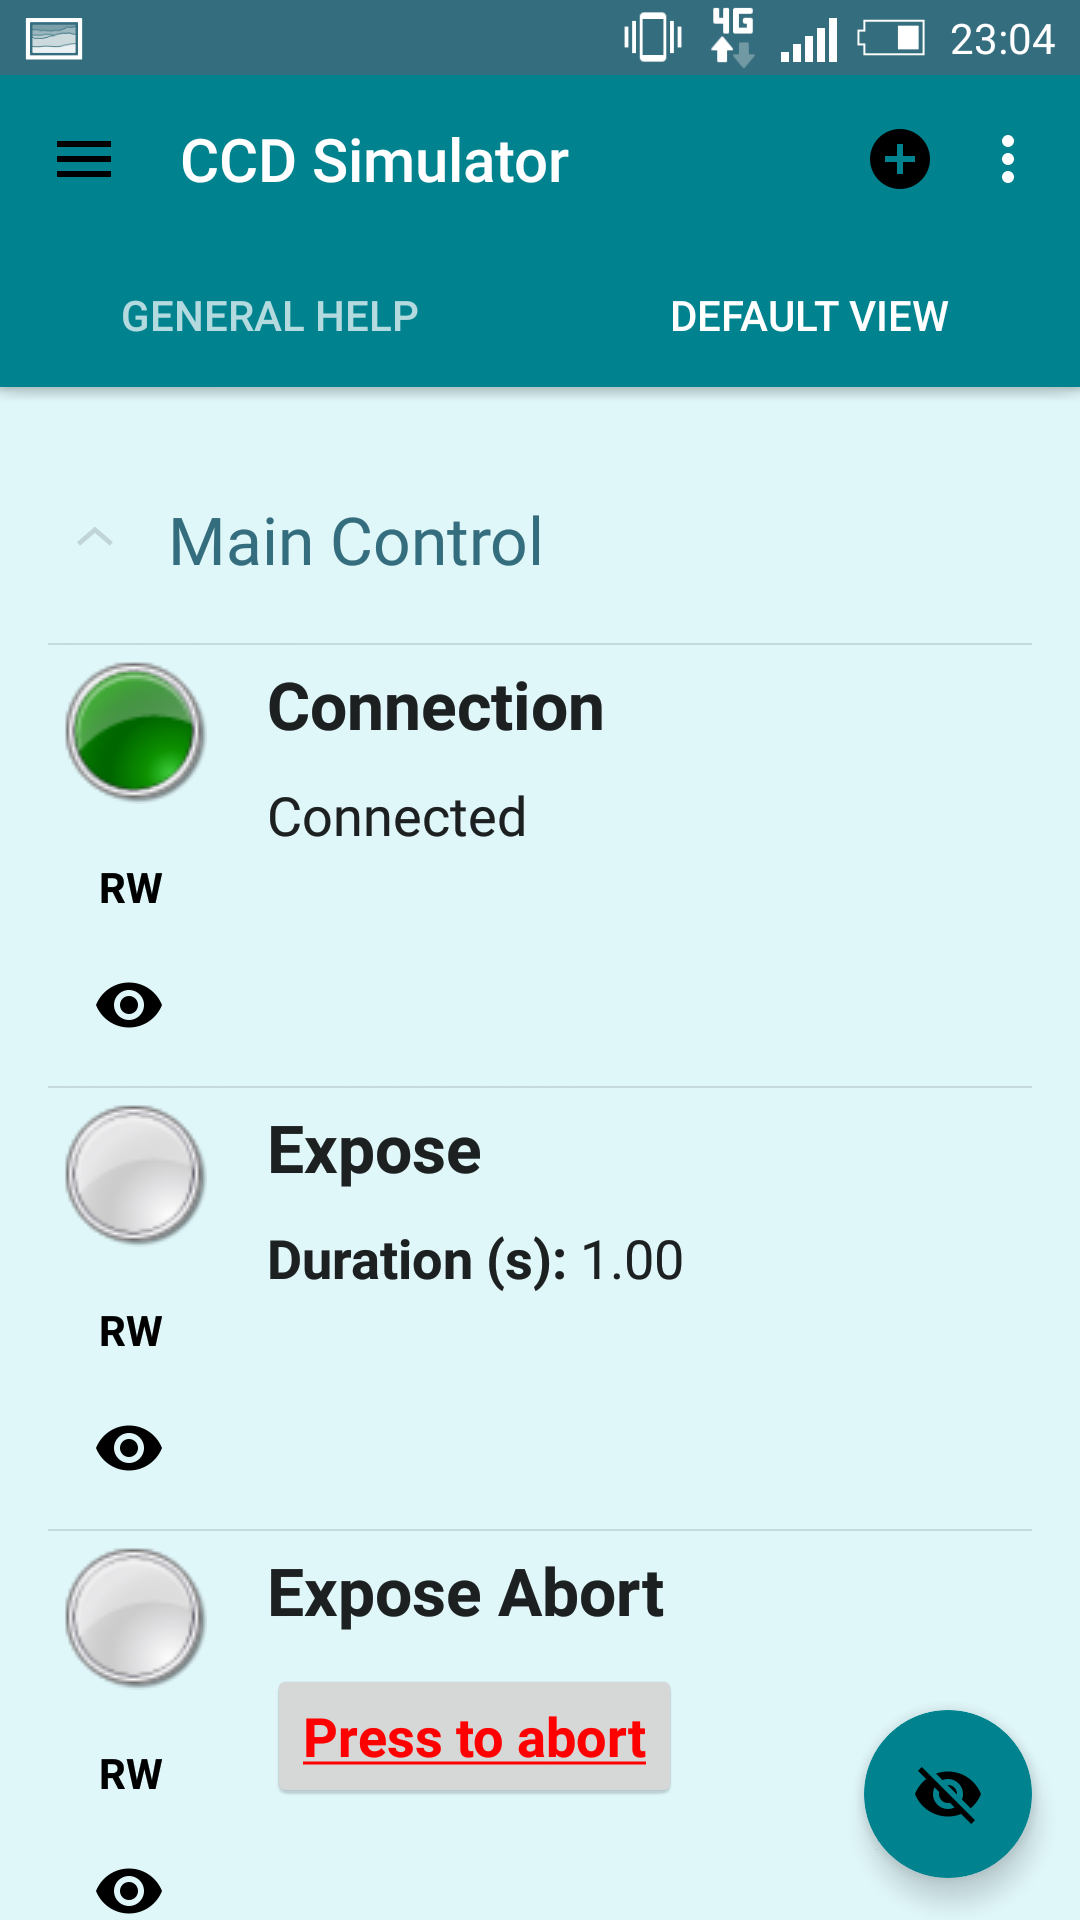
\includegraphics[width=0.3\textwidth]{../images/captura10.png}
  \caption{Vista de las propiedades connection y abort}
  \label{fig:connect_abort}
  \end{center}
\end{figure}

\begin{figure}[!ht]
  \begin{center}
  \includegraphics[width=0.3\textwidth]{../images/conncetion_property.png}
  \caption{Vista de edición para la propiedad Connection}
  \label{fig:connect_edit_view}
  \end{center}
\end{figure}

\begin{figure}[!ht]
  \begin{center}
  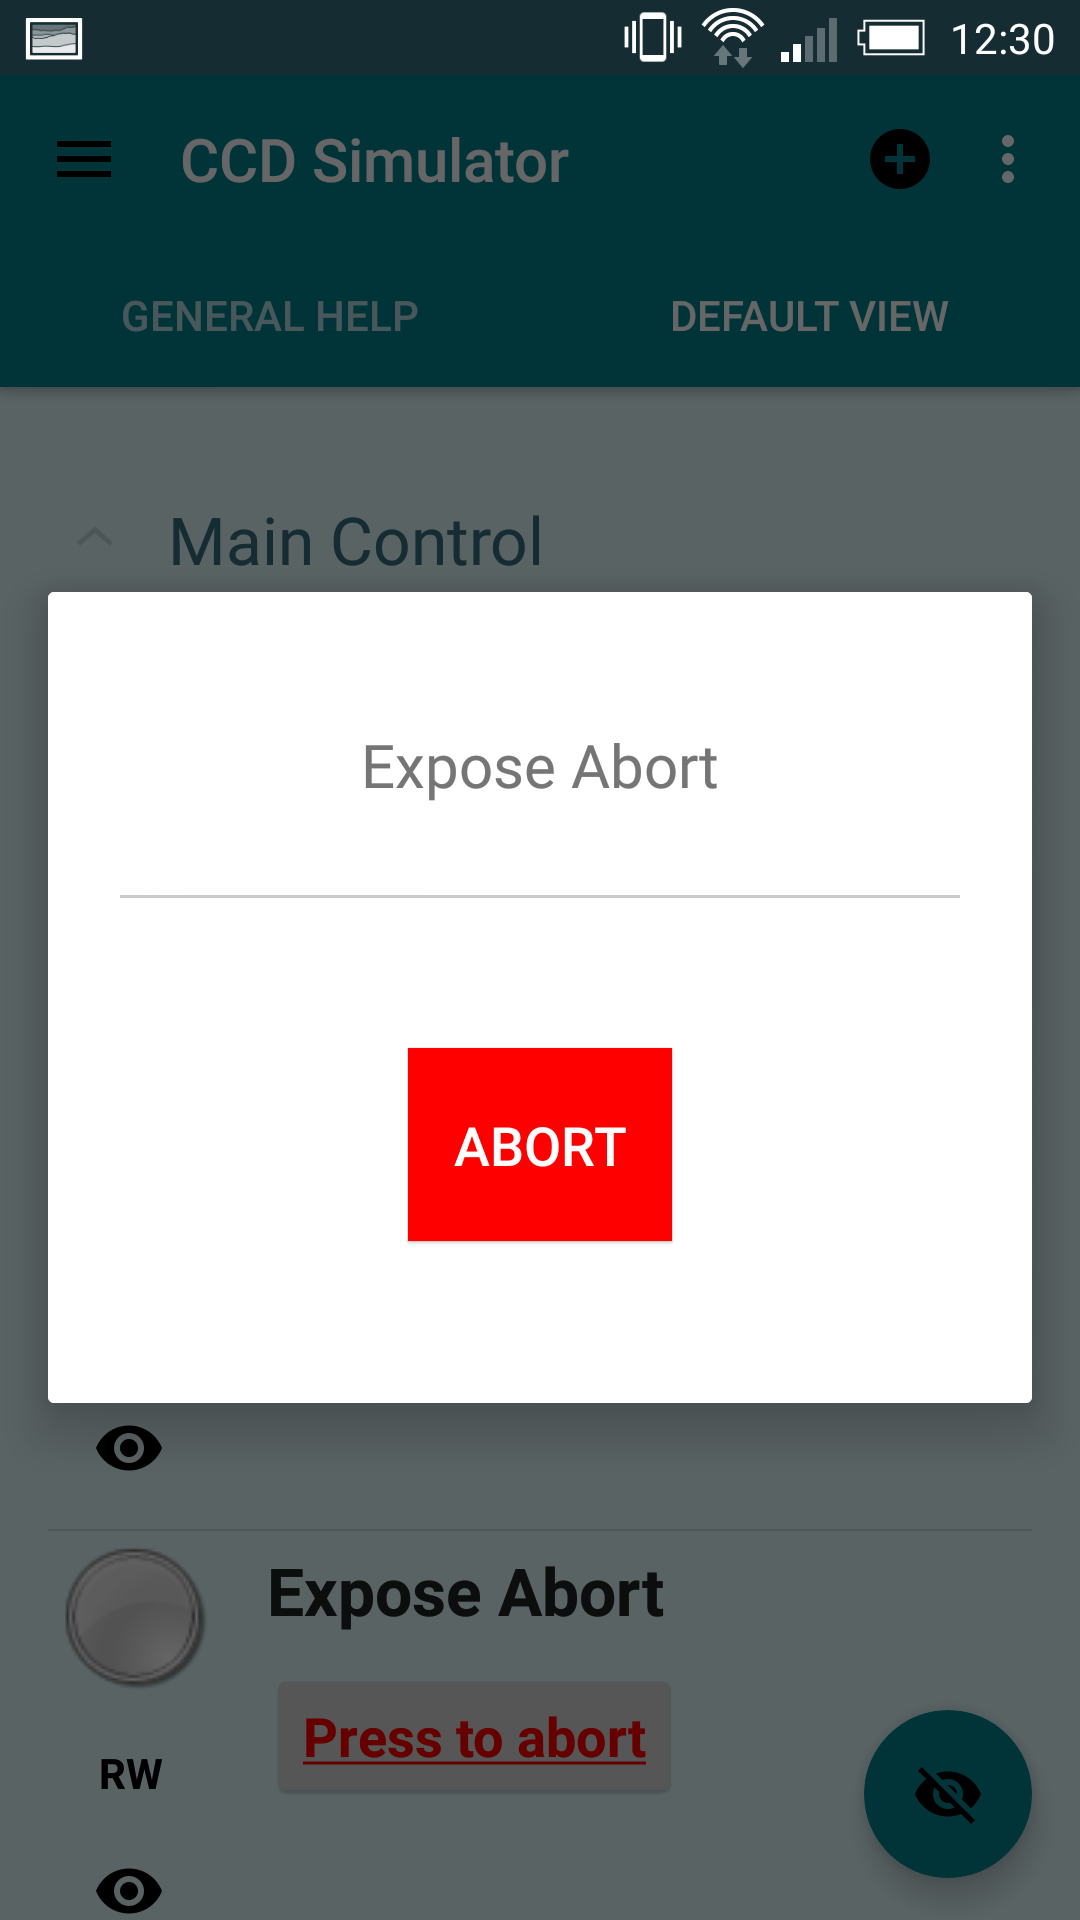
\includegraphics[width=0.3\textwidth]{../images/abort_property.png}
  \caption{Vista de edición para la propiedad Abort}
  \label{fig:connect_abort}
  \end{center}
\end{figure}

\newpage
\subsection{Dispositivos}
Al igual que con las propiedades, el software está diseñado para facilitar el diseño de nuevas clases para tener vistas especiales para algún dispositivo.

\bigskip
En el caso de las propiedades, se establecían prioridades para poder elegir de entre todas las posibilidades, cual iba a ser la interfaz de la propiedad concreta. En el caso de los dispositivos tenemos una interfaz de usuario por defecto, que lista las propiedades en una lista expandible. Pero se pueden añadir tantas como se deseen, pudiendo pasar de una a otra ya que se irían añadiendo al panel tabulado de la interfaz de usuario principal de la aplicación.

Para poder crear nuevas vistas para un dispositivo se ha diseñado la clase abstracta \texttt{DeviceView}.

\begin{lstlisting}[language=Java,caption={Clase abstracta DeviceView},label={lst:device_view}]
public abstract class DeviceView extends Fragment {

    static Device device;
    protected int layout;

    /**
     *  Check if this class can represent p
     *
     * @param dev Indi property
     * @return True/false if class can represent p
     */
    public abstract boolean handlesDevice (Device dev);

    public abstract String getName();

    @Override
    public abstract View onCreateView(LayoutInflater inflater, ViewGroup container, Bundle savedInstanceState);
}

\end{lstlisting}


\bigskip
Para poder crear una nueva vista de dispositivo debemos:

\begin{itemize}
  \item Crear una clase que herede de \texttt{deviceView}.
  \item Crear un archivo \textit{XML} con la definición de la interfaz de usuario.
  \item Añadir un objeto de la clase a la lista de clases manejadoras de dispositivos.
\end{itemize}


Como podemos ver en el fragmento de código \ref{lst:device_view}, tenemos dos atributos que son el dispositivo que vamos a manejar, y la referencia de \textbf{Android} al recurso donde se encuentra el archivo \textit{XML} con la definición de la vista. Además debemos implementar las siguientes funciones:


\begin{itemize}
  \item \texttt{handlesDevice}:
  Esta función recibe un dispositivo y debe comprobar si puede manejarlo o no devolviendo un valor booleano.

  \item \texttt{getName}:
  Esta función debe devolver el nombre que se desea que aparezca en la parte superior de la vista (vista tabulada).

  \item \texttt{onCreateView}:
  La clase abstracta hereda de \texttt{Fragment} y por ello esta función debe ser implementada, ya que se llamará cuando se llame a la clase para pintar la interfaz de usuario\cite{ALCA}. En ella deberemos crear la vista y realizar todas las inicializaciones que queramos.

\end{itemize}

\bigskip
En el fragmento de código \ref{} podemos ver una clase para mostrar una vista alternativa de una estación meteorológica concreta. Es una vista simple que muestra una imagen de fondo, pero es ilustrativa del proceso que debemos seguir para crear nuevas clases para manejar dispositivos.

\begin{lstlisting}[language=Java,caption={Clase abstracta DeviceView},label={lst:device_view}]
public class DeviceMeteoView extends DeviceView {
    @Override
    public boolean handlesDevice(Device dev) {
        if(dev.getName().equals("Meteo")){
            return true;
        }else
            return false;
    }

    @Override
    public String getName() {
        return "Meteo";
    }

    @Override
    public View onCreateView(LayoutInflater inflater, ViewGroup container, Bundle savedInstanceState) {
        layout=R.layout.meteo_view;
        View view = inflater.inflate(layout, container, false);
        FrameLayout frame=(FrameLayout)view.findViewById(R.id.layout);
        frame.setBackground(getResources().getDrawable(R.drawable.aagcloudwatcher));
        return view;
    }
}

\end{lstlisting}

\bigskip
Al igual que ocurría con las propiedades, debemos crear una vista definiéndola en un archivo \textit{XML} con los elementos visuales de \textbf{Android} que necesitemos.

\bigskip
Por último debemos agregar un objeto de nuestra clase a la lista de manejadores de dispositivos, como se ve en el fragmento de código \ref{lst:device_uis} llamando al método de la clase \texttt{Config} \texttt{addDeviceView(nuevo manejador)}

\begin{lstlisting}[language=Java,caption={Lista de objetos manejadores de dispositivos},label={lst:device_uis}]
private void setDeviceViews() {
    Config.addDeviceView(new DeviceMeteoView());
}

\end{lstlisting}